\documentclass[a4paper, 14pt, oneside]{extbook}
\usepackage[T1]{fontenc}
\usepackage[utf8x]{inputenc}
\usepackage{geometry}
\usepackage{courier}
\usepackage[bookmarks]{hyperref}
\newgeometry{
left=   1.5 in,
bottom= 1.5 in,
right=  1 in,
top=    1 in
}

\usepackage{fancyhdr}

% Grafica
\usepackage{graphicx,pstricks}
\usepackage{graphics}
\graphicspath{{img/}}

% Package usati per il frontespizio
\usepackage{tikz}
\usepackage{pgf-pie}
\usepackage{pgfplots}
\pgfplotsset{width=7cm,compat=1.8}
\usetikzlibrary{patterns}


%Algorithm
\usepackage{algorithm}
\usepackage[noend]{algpseudocode}

\setlength\headheight{44.2pt}
%Page Style
\usepackage{setspace}
%\setstretch{2.5} 
\doublespace

%\cfoot{\thepage}
\lhead[]{}
\rhead[]{\leftmark}

\pagestyle{fancy}{
\lhead{
\includegraphics[scale=0.3]{img/logo/hlogo.png}}
\rhead{\footnotesize{Titolo abbreviato come intestazione}}
}

%Other
\usepackage{comment}
\usepackage{amsmath}

%Testo riempitivo
\usepackage{lipsum}

%Titolo indice
\renewcommand*\contentsname{Indice}

%Inclusione bibliografia nell'indice
\renewcommand\bibname{Bibliografia}
\usepackage[nottoc,notlot,notlof]{tocbibind}

\begin{document}

%\maketitle
\begin{titlepage}
\thispagestyle{empty}
\raggedright % Allinea a sinistra

\begin{tikzpicture}
\node[anchor=south west] at (4,0) {
\includegraphics[scale=0.75]{img/logo/logo_copertina_1}};
\node[anchor=south west] at (0,1.5) {
\includegraphics{img/logo/logo_copertina_2}};
\node[anchor=south west] at (0,0.5) {\textsf{Scuola Politecnica e delle Scienze di Base}};
\node[anchor=south west] at (0,0) {\textsf{Corso di Laurea in Ingegneria Informatica}};
\end{tikzpicture}

\vfill

{\large Elaborato in \textbf{Architettura dei Sistemi Digitali}}
\\[1cm]
{\textbf{\textit{\LARGE Elaborato finale}}}
\\[1cm]
{\large Anno Accademico 2024/25}

\vfill


\begin{table}[h]
{\raggedright Studenti}
\\
\textbf{Filomena Vigliotti}
\\
\textbf{matr. M63001734}
\\
\textbf{Ciro Scognamilgio}
\\
\textbf{matr. M6300}
\\
\textbf{Antonio Sirignano}
\\
\textbf{matr. M63001732}
\end{table}

\end{titlepage}
\frontmatter

%\cleardoublepage
%\thispagestyle{empty}
\vspace*{\stretch{1}}
\begin{flushright}
\itshape Una dedica...
\end{flushright}
\vspace{\stretch{2}}
\cleardoublepage

{\setstretch{1.5}
\tableofcontents
}

\mainmatter

\chapter*{Introduzione}

\addcontentsline{toc}{chapter}{Introduzione}

\lipsum[1-3]

% Esempio di citazioni bibliografiche - vedi file "bibliography.bib"
\cite{librocitato}
\cite{articolocitato}
\cite{articoloconferenza}
\cite{sitocitato}
\chapter{Problema 1}

\section{Multiplexer 16:1}

\subsection{Multiplexer indirizzabile 16:1}
Si chiede di progettare un multiplexer indirizzabile 16:1, utilizzando un approccio per composizione, utilizzando multiplexer 4:1.\\
Quindi quello che si vuole progettare è il multiplexer rappresentato come seguito.
\begin{figure}[H]
	\centering
	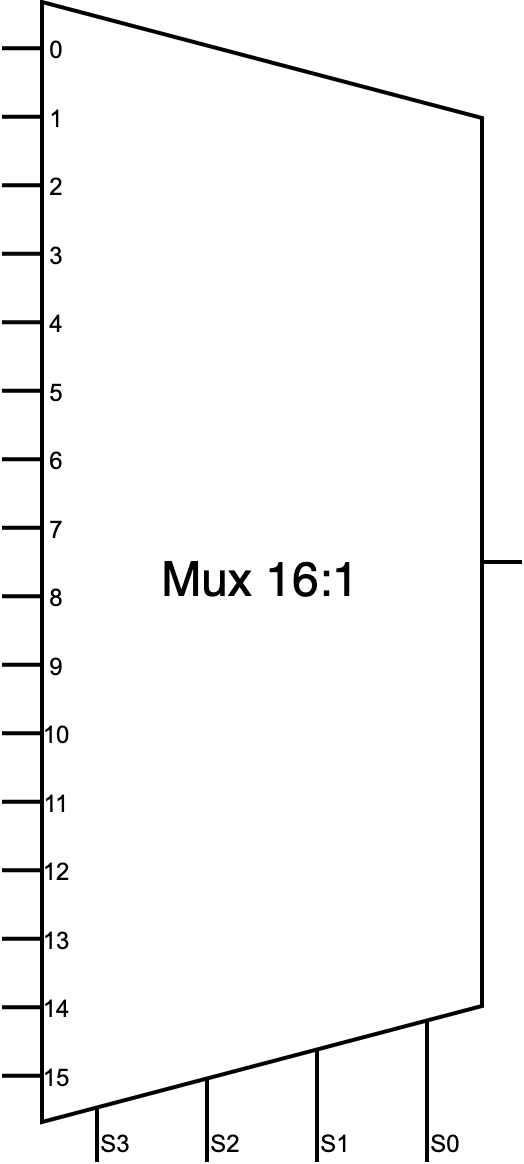
\includegraphics[width=0.2\textwidth]{img/01}
	\label{01} 
\end{figure}
Utilizzando l'approccio per composizione, si vuole dapprima progettare un multiplexer 4:1, utilizzando tre multiplexer 2:1.


\subsection{Rete di interconnessione a 16 ingressi e 4 uscite}

\subsection{Implementazione su board}

\section{Esercizio 1 - Sistema ROM+M}

\chapter{Title}

\lipsum[1][1-3]

\section{Section ...}

\lipsum
\chapter{Title}

\lipsum[1][1-3]

\section{Section ...}

\lipsum
\include{chapter4}
\include{chapter5}
\include{chapter6}
\include{chapter7}
\include{chapter8}

\chapter{Conclusioni}

\lipsum[23]


\bibliography{bibliography}
\bibliographystyle{plain}

\end{document}